\section{Parser}
Once the lexer has recognized input, the parser is in charge of handling said input. For example, if the lexer recognizes an \textit{or}-expression, the parser must determine if the semantics are in order - for example if the \textit{or}-operator is used, it must check if the operator is used on two expressions in a proper maner. If not, the parser must recognize this and a parsing-error will occur. Returning to the \textit{or}-operator, it only makes sense if the \textit{or}-keyword is sandwiched between two expressions or else the use of the \textit{or}-operator doesn't fit its formal definition. The parser checks if this is the case, and if so, calls upon the typechecker to ensure the types of the expressions are in order. The check, which the parser makes, looks like this in our implementation:\\
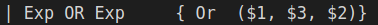
\includegraphics[width=\linewidth]{Materials/Parser/Or}\\
This implementation ensures that only the \textit{or}-operator when sandwiched between two expressions is accepted, or else an error will be raised. 
